\section{Null\-Buffer Class Reference}
\label{classNullBuffer}\index{NullBuffer@{NullBuffer}}
Inheritance diagram for Null\-Buffer::\begin{figure}[H]
\begin{center}
\leavevmode
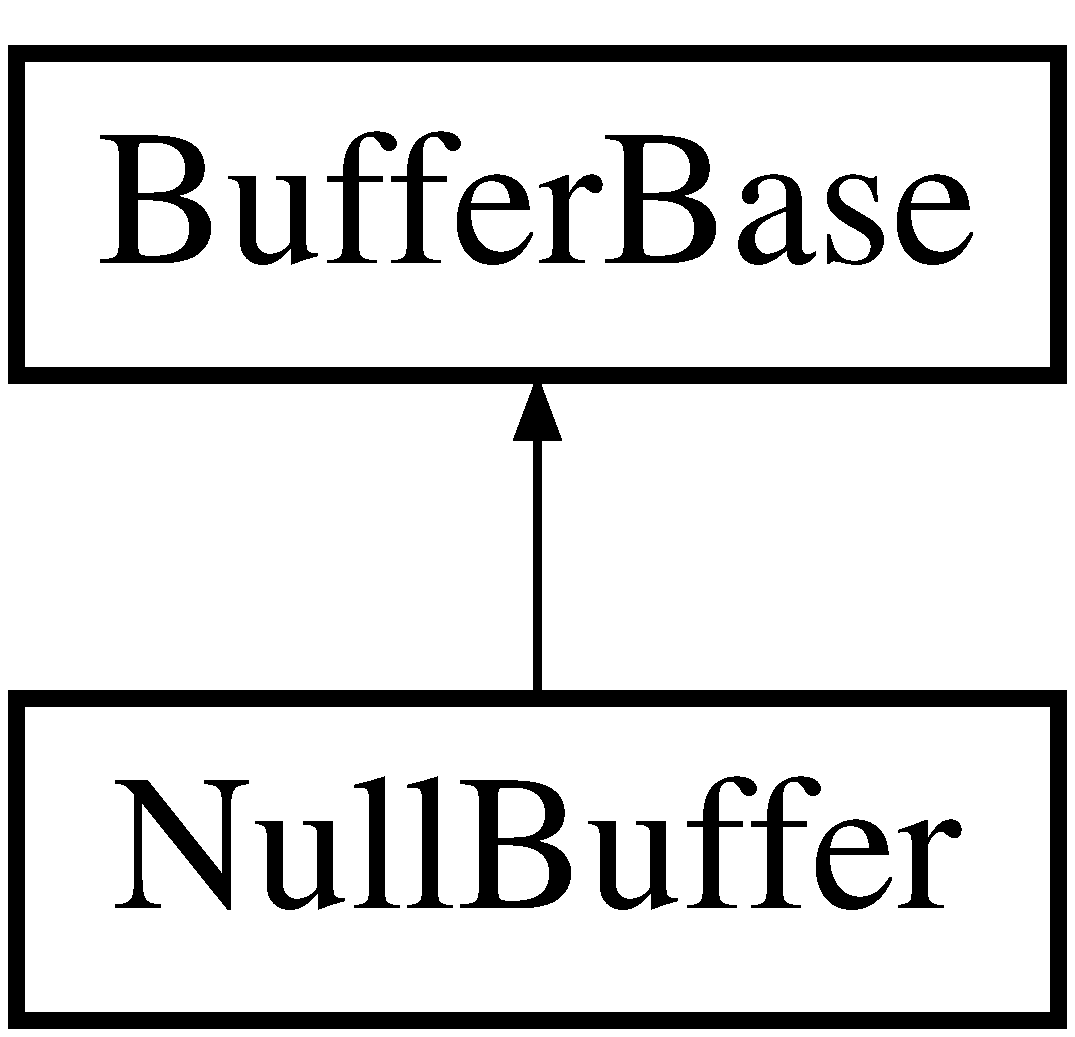
\includegraphics[height=2cm]{classNullBuffer}
\end{center}
\end{figure}
\subsection*{Public Member Functions}
\begin{CompactItemize}
\item 
{\bf \_\-\_\-init\_\-\_\-} (size=None)
\item 
{\bf init} (data)
\item 
{\bf clear} ()
\item 
{\bf length} ()
\begin{CompactList}\small\item\em Get the buffer length. \item\end{CompactList}\item 
{\bf write} (value)
\begin{CompactList}\small\item\em Write data into the buffer. \item\end{CompactList}\item 
{\bf read} (value)
\begin{CompactList}\small\item\em Read data from the buffer. \item\end{CompactList}\item 
{\bf is\-Full} ()
\begin{CompactList}\small\item\em True if the buffer is full, else false. \item\end{CompactList}\item 
{\bf is\-Empty} ()
\begin{CompactList}\small\item\em True if the buffer is empty, else false. \item\end{CompactList}\item 
{\bf is\-New} ()
\item 
{\bf put} (data)
\begin{CompactList}\small\item\em Write data into the buffer. \item\end{CompactList}\item 
{\bf get} ()
\begin{CompactList}\small\item\em Get data from the buffer. \item\end{CompactList}\item 
{\bf get\-Ref} ()
\begin{CompactList}\small\item\em Get the buffer's reference to be written the next. \item\end{CompactList}\item 
{\bf \_\-\_\-init\_\-\_\-} ()
\end{CompactItemize}


\subsection{Member Function Documentation}
\index{NullBuffer@{Null\-Buffer}!__init__@{\_\-\_\-init\_\-\_\-}}
\index{__init__@{\_\-\_\-init\_\-\_\-}!NullBuffer@{Null\-Buffer}}
\subsubsection{\setlength{\rightskip}{0pt plus 5cm}Buffer\-Base::\_\-\_\-init\_\-\_\- ()\hspace{0.3cm}{\tt  [inherited]}}\label{classBufferBase_NullBuffera12}


\index{NullBuffer@{Null\-Buffer}!__init__@{\_\-\_\-init\_\-\_\-}}
\index{__init__@{\_\-\_\-init\_\-\_\-}!NullBuffer@{Null\-Buffer}}
\subsubsection{\setlength{\rightskip}{0pt plus 5cm}Null\-Buffer::\_\-\_\-init\_\-\_\- (size = {\tt None})}\label{classNullBuffer_NullBuffera0}


\index{NullBuffer@{Null\-Buffer}!clear@{clear}}
\index{clear@{clear}!NullBuffer@{Null\-Buffer}}
\subsubsection{\setlength{\rightskip}{0pt plus 5cm}Null\-Buffer::clear ()}\label{classNullBuffer_NullBuffera2}


\index{NullBuffer@{Null\-Buffer}!get@{get}}
\index{get@{get}!NullBuffer@{Null\-Buffer}}
\subsubsection{\setlength{\rightskip}{0pt plus 5cm}Null\-Buffer::get ()}\label{classNullBuffer_NullBuffera10}


Get data from the buffer. 



Reimplemented from {\bf Buffer\-Base} {\rm (p.\,\pageref{classBufferBase_BufferBasea7})}.\index{NullBuffer@{Null\-Buffer}!getRef@{getRef}}
\index{getRef@{getRef}!NullBuffer@{Null\-Buffer}}
\subsubsection{\setlength{\rightskip}{0pt plus 5cm}Null\-Buffer::get\-Ref ()}\label{classNullBuffer_NullBuffera11}


Get the buffer's reference to be written the next. 



Reimplemented from {\bf Buffer\-Base} {\rm (p.\,\pageref{classBufferBase_BufferBasea8})}.\index{NullBuffer@{Null\-Buffer}!init@{init}}
\index{init@{init}!NullBuffer@{Null\-Buffer}}
\subsubsection{\setlength{\rightskip}{0pt plus 5cm}Null\-Buffer::init (data)}\label{classNullBuffer_NullBuffera1}


\index{NullBuffer@{Null\-Buffer}!isEmpty@{isEmpty}}
\index{isEmpty@{isEmpty}!NullBuffer@{Null\-Buffer}}
\subsubsection{\setlength{\rightskip}{0pt plus 5cm}Null\-Buffer::is\-Empty ()}\label{classNullBuffer_NullBuffera7}


True if the buffer is empty, else false. 



Reimplemented from {\bf Buffer\-Base} {\rm (p.\,\pageref{classBufferBase_BufferBasea5})}.\index{NullBuffer@{Null\-Buffer}!isFull@{isFull}}
\index{isFull@{isFull}!NullBuffer@{Null\-Buffer}}
\subsubsection{\setlength{\rightskip}{0pt plus 5cm}Null\-Buffer::is\-Full ()}\label{classNullBuffer_NullBuffera6}


True if the buffer is full, else false. 



Reimplemented from {\bf Buffer\-Base} {\rm (p.\,\pageref{classBufferBase_BufferBasea4})}.\index{NullBuffer@{Null\-Buffer}!isNew@{isNew}}
\index{isNew@{isNew}!NullBuffer@{Null\-Buffer}}
\subsubsection{\setlength{\rightskip}{0pt plus 5cm}Null\-Buffer::is\-New ()}\label{classNullBuffer_NullBuffera8}


\index{NullBuffer@{Null\-Buffer}!length@{length}}
\index{length@{length}!NullBuffer@{Null\-Buffer}}
\subsubsection{\setlength{\rightskip}{0pt plus 5cm}Null\-Buffer::length ()}\label{classNullBuffer_NullBuffera3}


Get the buffer length. 



Reimplemented from {\bf Buffer\-Base} {\rm (p.\,\pageref{classBufferBase_BufferBasea1})}.\index{NullBuffer@{Null\-Buffer}!put@{put}}
\index{put@{put}!NullBuffer@{Null\-Buffer}}
\subsubsection{\setlength{\rightskip}{0pt plus 5cm}Null\-Buffer::put (data)}\label{classNullBuffer_NullBuffera9}


Write data into the buffer. 



Reimplemented from {\bf Buffer\-Base} {\rm (p.\,\pageref{classBufferBase_BufferBasea6})}.\index{NullBuffer@{Null\-Buffer}!read@{read}}
\index{read@{read}!NullBuffer@{Null\-Buffer}}
\subsubsection{\setlength{\rightskip}{0pt plus 5cm}Null\-Buffer::read (value)}\label{classNullBuffer_NullBuffera5}


Read data from the buffer. 



Reimplemented from {\bf Buffer\-Base} {\rm (p.\,\pageref{classBufferBase_BufferBasea3})}.\index{NullBuffer@{Null\-Buffer}!write@{write}}
\index{write@{write}!NullBuffer@{Null\-Buffer}}
\subsubsection{\setlength{\rightskip}{0pt plus 5cm}Null\-Buffer::write (value)}\label{classNullBuffer_NullBuffera4}


Write data into the buffer. 



Reimplemented from {\bf Buffer\-Base} {\rm (p.\,\pageref{classBufferBase_BufferBasea2})}.

The documentation for this class was generated from the following file:\begin{CompactItemize}
\item 
{\bf Buffer\-Base.py}\end{CompactItemize}
